\documentclass{article}
\usepackage{graphicx}
\usepackage{amsmath}


\title{Exercise 8}
\author{Joanna Brodbeck}
\date{\today}

\begin{document}

\maketitle

\section{Color Modes}
\subsubsection*{How do you transform a specification in RGB into CMY?}
\textbf{Rgb} color space consists of all possible colors that can be made by the combination of red, green, and blue light. It's a popular model in photography, television, and computer graphics.\\
\begin{center}
    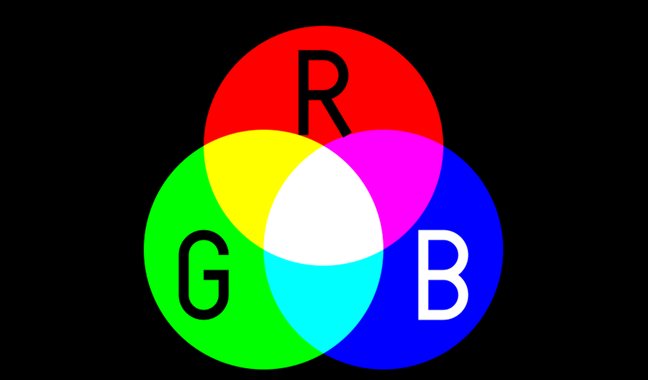
\includegraphics[width=0.5\textwidth]{assets/rgb.png}
\end{center}
\textbf{Cmy} is frequency associated with color printing, and it's determined by the relation of colors cyan, magenta and yellow. Unlike Rgb, cmy is subtractive, meaning that higher values are associated with darker colors rather than light.
\begin{center}
    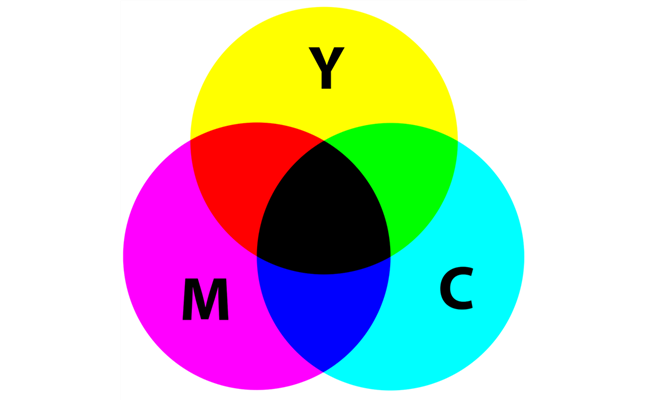
\includegraphics[width=0.5\textwidth]{assets/ymc.png}
\end{center}
\[
C = 1 - R
\]
\[
M = 1 - G
\]
\[
Y = 1 - B
\]
Here, \( R \), \( G \), and \( B \) represent the normalized values of the Red, Green, and Blue components, respectively. The values of \( C \), \( M \), and \( Y \) will be in the range [0, 1], where 0 corresponds to no color and 1 corresponds to full color intensity.

\subsubsection*{Why were color spaces such as RGB, CMY, YIQ, and HSL specified, and
    where are they being applied?}
\paragraph*{RGB}
\begin{itemize}
    \item illuminated screens (TV, laptop, smartphone)
    \item software
    \item sum up to white
    \item Additive color space used for color monitors
    \item Neighboring color pixels are mixed to one color by the human eye
\end{itemize}

\paragraph*{CMY}
\begin{itemize}
    \item printing
    \item sum up to black
    \item subtractive color model
\end{itemize}

\paragraph*{YIQ}
\begin{itemize}
    \item TV (NTSC)
    \item human perception
    \item Y: luminance (brightness)
    \item I: in-phase (color information)
    \item Q: quadrature (color information)
    \item Separation allows more efficient compression and transmission of color information.
\end{itemize}

\paragraph*{HSL}
\begin{itemize}
    \item human perception (hue = type of color)
    \item saturation (intensity of purity of color)
    \item lightness (brightness)
    \item graphic design, image editing software providing a more intuitive way to adjust colors.
\end{itemize}
\subsubsection*{Provide the values for a medium gray in the following color modes: RGB,
    CMY, YIQ and HSV.}
\paragraph*{RGB}
\begin{itemize}
    \item R = 0.5
    \item G = 0.5
    \item B = 0.5
\end{itemize}

\paragraph*{CMY}
\begin{itemize}
    \item C = 0.5
    \item M = 0.5
    \item Y = 0.5
\end{itemize}

\paragraph*{CMYK}
\begin{itemize}
    \item C = 0
    \item M = 0
    \item Y = 0
    \item K = 0.5
\end{itemize}

\paragraph*{YIQ}
\begin{itemize}
    \item Y = 0.5
    \item I = 0
    \item Q = 0
\end{itemize}

\paragraph*{HSV}
\begin{itemize}
    \item H = 0
    \item S = 0
    \item V = 0.5
\end{itemize}



\section{RGB Color Space and White Point Calibration
 }

The RGB color space is a subspace of the XYZ color space. Assume the base
vectors are directly related to the used phosphors often used in monitors, also
known as ITU-R BT.709-standard. The color components \(x\) and \(y\) of the RGB
base vectors are given in the table below.

\begin{table}[h]
    \centering
    \begin{tabular}{c|c|c|c}
          & R    & G    & B    \\ % Remove the extra alignment tab here
        \hline
        X & 0.64 & 0.30 & 0.15 \\
        \hline
        Y & 0.33 & 0.60 & 0.06 \\
    \end{tabular}
    \caption{RGB Base Vectors}
\end{table}

The white point is identified as (0.9505, 1.0000, 1.0890).

\subsubsection*{Name one advantage and one disadvantage of the RGB color space. Furthermore, list one color space each, which does not have this advantage or
    disadvantage.}

\paragraph*{Advantage}
\begin{itemize}
    \item useful for monitors and displays
    \item RGB is an additive color model, meaning that the colors are added together in various ways to reproduce a broad array of colors.
    \item YIQ is a color space that is not additive and has thus less colors.
\end{itemize}

\paragraph*{Disadvantage}
\begin{itemize}
    \item color mixing is not intuitive (in contrary to HLS, HSV)
    \item not useful for printing
    \item RGB is device-dependent, meaning that the color space is defined by the characteristics of a particular device such as your computer monitor or television screen.
    \item HSL is device-independent, meaning that the color space is defined independent of the device.
\end{itemize}
\subsubsection*{Evaluate the z-component of the RGB-base vectors.}

\begin{table}[h]
    \centering
    \begin{tabular}{c|c|c|c}
         & R    & G    & B    \\ % Remove the extra alignment tab here
        \hline
        $Z = 1 - X - Y$ & 0.03 & 0.10 & 0.79 \\
    \end{tabular}
    \caption{RGB Base Vectors}
\end{table}
\begin{align*}
    X (R) &= 0.64 \\
    Y (R)&= 0.33 \\
    Z (R) &= 1 - 0.64 - 0.33 = 0.03 \\
\end{align*}
The RGB values (X, Y, Z) are related to the XYZ values (X, Y, Z) by the following equation:
\[
\begin{bmatrix} X \\ Y \\ Z \end{bmatrix} = \begin{bmatrix} R_X & G_X & B_X \\ R_Y & G_Y & B_Y \\ R_Z & G_Z & B_Z \end{bmatrix} \times \begin{bmatrix} R \\ G \\ B \end{bmatrix}
\]
Now, we can evaluate the z-component of the RGB base vectors:
\[
Z = 1 - X - Y
\]
For each base vector:
\[
Z_R = 1 - 0.64 - 0.33 = 0.03
\]
\[
Z_G = 1 - 0.30 - 0.60 = 0.10
\]
\[
Z_B = 1 - 0.15 - 0.06 = 0.79
\]
So, the z-components of the RGB base vectors are approximately 0.03, 0.10, and 0.79 for R, G, and B, respectively.
\subsubsection*{Provide the equation system for the white point calibration. Name the calibration parameters $C_R$, $C_G$ and $C_B$.}
Given the RGB values (X, Y, Z) and the white point (0.9505, 1.0000, 1.0890), we can find the matrix and then evaluate the z-component of the RGB base vectors.
\[
\begin{bmatrix} X \\ Y \\ Z \end{bmatrix} = \begin{bmatrix} 0.64 & 0.30 & 0.15 \\ 0.33 & 0.60 & 0.06 \\ \text{?} & \text{?} & \text{?} \end{bmatrix} \times \begin{bmatrix} R \\ G \\ B \end{bmatrix}
\]
Since the white point is (0.9505, 1.0000, 1.0890), we can use this information to find the missing values in the matrix.
\[
\begin{bmatrix} 0.9505 \\ 1.0000 \\ 1.0890 \end{bmatrix} = \begin{bmatrix} 0.64 & 0.30 & 0.15 \\ 0.33 & 0.60 & 0.06 \\ \text{?} & \text{?} & \text{?} \end{bmatrix} \times \begin{bmatrix} R \\ G \\ B \end{bmatrix}
\]
Solving this system of equations, we get:
\[
\begin{bmatrix} R \\ G \\ B \end{bmatrix} = \begin{bmatrix} 1.0232 \\ 1.0000 \\ 0.6863 \end{bmatrix}
\]

\subsubsection{Suppose $C_R = 0.6445$, $C_G = 1.1919$, and $C_B = 1.2031$ are given as a solution. Evaluate the transformation matrix from the linear color space RGB into the color space XYZ.}

\section{Color Space Transformation}
In this exercise we focus on the transformation from colors in the sRGB-color space
into the broadly known color spaces used in television, namely PAL and NTSC.
In order to be compatible with old black and white systems, the first channel
of the PAL-color space (also known as YUV-color space) is the Y-coordinate
of the XYZ-color space. Since the Y-coordinate
\[ Y = 0.2126 \cdot R + 0.7152 \cdot G + 0.0722 \cdot B \]
contains a major green component, \( C_b \) and \( C_r \) are chosen in a way such that
they contain a major blue respectively red component:
\[ C_b = B - Y, \quad C_r = R - Y \]
Finally, normalizing the \(C_b\) and \(C_r\) channels leads to the YUV- or PAL-color space:
\[ U = 0.49 \cdot C_b, \quad V = 0.88 \cdot C_r \]

\subsubsection*{Provide the transformation matrix from the sRGB-color space into the YUVcolor space.}
To derive the transformation matrix from the sRGB color space to the YUV (PAL) color space, we can use the provided formulas for Y, Cb, and Cr, and then express them in matrix form. The sRGB color space is typically represented as a linear transformation of the RGB values. The transformation matrix can be denoted as:

\[ \begin{bmatrix} Y \\ C_b \\ C_r \end{bmatrix} = \begin{bmatrix} a & b & c \\ d & e & f \\ g & h & i \end{bmatrix} \begin{bmatrix} R \\ G \\ B \end{bmatrix} \]

Substituting the given equations for Y, Cb, and Cr into this matrix equation, we can solve for the elements of the matrix. The equations are:

\[ Y = 0.2126 \cdot R + 0.7152 \cdot G + 0.0722 \cdot B \]
\[ C_b = B - Y \]
\[ C_r = R - Y \]
\[ C_b = B - Y \]
Substituting the expression for \( Y \):
\[ C_b = B - (0.2126 \cdot R + 0.7152 \cdot G + 0.0722 \cdot B) \]
Simplifying further:
\[ C_b = -0.2126 \cdot R - 0.7152 \cdot G + 0.9278 \cdot B \]
Now, the correct transformation matrix from the sRGB color space to the YUV (PAL) color space is:
\[ \begin{bmatrix} Y \\ U \\ V \end{bmatrix} = \begin{bmatrix} 0.2126 & 0.7152 & 0.0722 \\ -0.2126 & -0.7152 & 0.9278 \\ 0.7874 & -0.7152 & -0.0722 \end{bmatrix} \begin{bmatrix} R \\ G \\ B \end{bmatrix} \]

\subsubsection*{The YIQ- or NTSC-color space is used as the US television standard. It is
created from the PAL color space, by swapping the U- and V-coordinates followed by a rotation by 33 degrees around Y-axis. Evaluate the transformation
matrix for the conversion from PAL to NTSC. You do not have to evaluate
trigonometric expressions}
\paragraph*{Rotation Matrix}
\[
\begin{bmatrix}
1 & 0 & 0 \\
0 & \cos(33^\circ) & -\sin(33^\circ) \\
0 & \sin(33^\circ) & \cos(33^\circ)
\end{bmatrix}
\]



\[ \begin{bmatrix} Y_{\text{NTSC}} \\ I_{\text{NTSC}} \\ Q_{\text{NTSC}} \end{bmatrix} = \begin{bmatrix} 1 & 0 & 0 \\ 0 & \sin(33^\circ) & \cos(33^\circ) \\ 0 & \cos(33^\circ) & -\sin(33^\circ) \end{bmatrix} \begin{bmatrix} Y_{\text{PAL}} \\ V_{\text{PAL}} \\ U_{\text{PAL}} \end{bmatrix} \]


\subsubsection*{The YIQ-channels are splitting the bandwidth proportional to 8:5:2 during
the transfer of NTSC color signals. Why is such an uneven bandwidth being
used?}
When the NTSC standard was developed, it needed to work within the limitations of the existing technology, including the available transmission bandwidth. The 8:5:2 ratio struck a balance between providing good image quality and fitting within the constraints of the available broadcast spectrum.
\section{CIE-Chart}
\subsubsection*{Which properties does a mixed color in the CIE-Chart have to its primaries?}

\subsubsection*{Which meaning does the connection between 770nm and 380nm have in this chart?}
\begin{itemize}
    \item The connection between 770nm and 380nm is the visible spectrum of light.
\end{itemize}

\subsubsection*{The figure below shows a CIE-Chart. Add the following primaries into the chart.}

\begin{center}  
\begin{tabular}{c|c|c|c}
    \text{Primaries} & x & y & Y \\
    \hline
    C1 & 0.1 & 0.8 & 12 \\
    \hline
    C2 & 0.6 & 0.3 & 26 \\
    \hline
    C3 & 0.2 & 0.05 & 10 \\
\end{tabular}
\end{center}

\subsubsection*{Determine the dominant wavelengths \( \lambda_1, \lambda_2, \) and \( \lambda_3 \) of the 3 primaries.}

\subsubsection*{For each primary, draw the isoline of constant saturation passing through it into the chart.}

\subsubsection*{Determine the primary C123, which is the sum (in the XYZ-space) of the 3 primaries C1, C2, and C3. Add it to the chart.}

\subsubsection*{Can al Spectral Colors with Full Saturation be Mixed from Three Linearly Independent Primaries?}

\end{document}
\end{document}
